
% LTeX: language=en

% wordcloud : draw word cloud with MetaPost and Lua
%
% Originally written by Maxime Chupin <notezik@gmail.com>,
% 2023.
%

\documentclass[english]{ltxdoc}

\usepackage{tcolorbox}
\tcbuselibrary{listings,breakable}
%\tcbuselibrary{documentation}
\usepackage{enumitem}
\usepackage[tikz]{bclogo}
\usepackage{mflogo}
\usepackage{hologo}
\usepackage{luamplib}
\mplibtextextlabel{enable}
\usepackage{biblatex}
\addbibresource{ctan.bib}
\usepackage{wrapfig}
\usepackage{accsupp}
\usepackage{siunitx}
\usepackage{imakeidx}
%\usepackage{csquotes}
\usepackage{fancyvrb,xparse,xargs}
\usepackage[sfdefault]{FiraSans}
\usepackage[mathrm=sym]{firamath-otf}
\setmonofont{Fira Mono}
%\setmonofont{FiraCode-Regular.ttf}[BoldFont= FiraCode-Bold.ttf,ItalicFont= FiraCode-RegularItalic.otf,BoldItalicFont= FiraCode-BoldItalic.otf,Ligatures={NoCommon, NoDiscretionary, NoHistoric, NoRequired, NoContextual}]

\usepackage{xspace}
\usepackage{animate}
\newcommand{\ctan}{\textsc{ctan}}
\NewDocumentCommand{\package}{ m }{%
  \href{https://ctan.org/pkg/#1}{#1}\xspace
}

\definecolor{darkred}{rgb}{0.6,0.1,0.1}
\definecolor{vert}{rgb}{0.1,0.4,0.1}
\definecolor{bleu}{rgb}{0.2,0.2,0.6}
\definecolor{orange}{rgb}{0.6,0.4,0.}
\colorlet{code}{blue!80!black}

\usepackage[colorlinks=true,urlcolor=orange,linkcolor=orange,menucolor=black,citecolor=orange]{hyperref}

\newcommand \file       {\nolinkurl}
\renewcommand \cmd        {\texttt}
\renewcommand \code   [1] {\texorpdfstring {\texttt{\color{code}#1}} {#1}}
\renewcommand*\cs     [1] {\code{\textbackslash #1}}



\newcommand*\commande{\par\bigskip\noindent\hspace{-30pt}%
  \SaveVerb[aftersave={%
   \UseVerb{Vitem}%
  }%
  ]{Vitem}%
  }
  \newcommand\vitem[1][]{\SaveVerb[%
  aftersave={\item[\textnormal{\UseVerb[#1]{vsave}}]}]{vsave}}
\newcommand*\textme[1]{\textcolor{black}{\rmfamily\textit{#1}}}
%\renewcommand*\meta[1]{% % meta
%  \textme{\ensuremath{\langle}#1\ensuremath{\rangle}}}
\newcommand*\optstar{% % optional star
  \meta{\ensuremath{*}}\xspace}
\DefineShortVerb{\|}
\newcommand\R{\mathbf{R}}
\setlength{\fboxsep}{2pt}
\fvset{%
  codes={\catcode`\«\active \catcode`\×\active },
  defineactive={\makefancyog\makefancytimes},
  formatcom=\color{darkred},
  frame=single
}
% rendre «...» équivalent à \meta{...}
{\catcode`\«\active
  \newcommandx\makefancyog[0][addprefix=\global]{%
    \def«##1»{\meta{##1}}}}
% rendre × équivalent à \optstar
{\catcode`\×\active
  \newcommandx\makefancytimes[0][addprefix=\global]{%
    \def×{\optstar{}}}}


\newcommand\wordcloudpkg{\texttt{wordcloud}\xspace}

\def\MO/{{\fontspec{fetamont}META\-OBJ}}

%\addbibresource{biblio.bib}


\lstset{
  numberstyle=\footnotesize\color{vert},
  keywordstyle=\ttfamily\bfseries\color{bleu},
  basicstyle=\ttfamily,
  commentstyle=\itshape\color{vert},
  stringstyle=\ttfamily\color{orange},
  showstringspaces=false,
  language=MetaPost,
  breaklines=true,
  breakindent=30pt,
  defaultdialect=MetaPost,
  classoffset=1,% frame=tb
  morekeywords={},
  keywordstyle=\color{darkred},
  classoffset=2,% frame=tb
  morekeywords={backboard,chessboard,chessboard_step},
  keywordstyle=\color{vert},
  classoffset=0,% frame=tb
  morekeywords={draw},
  keywordstyle=\color{bleu}
}


\extractcolorspecs{darkred!3}\modelcmd\colorcmd
\makeatletter
\tcbset{%
    listing metapost/.code={%
        \def\tcbuselistingtext@input{\begin{mplibcode}     verbatimtex \leavevmode etex;
          background:=(\colorcmd); input \jobname.listing; \end{mplibcode}}%
    }
}
\makeatother
\newtcblisting[auto counter,]{ExempleMP}[1][]{%
  arc=0pt,outer arc=0pt,
  colback=darkred!3,
  colframe=darkred,
  breakable,fontupper=\small,
  boxsep=0pt,left=5pt,right=5pt,top=5pt,bottom=5pt, bottomtitle =
  3pt, toptitle=3pt,
  boxrule=0pt,bottomrule=0.5pt,toprule=0.5pt, toprule at break =
  0pt, bottomrule at break = 0pt,
  %listing side text,
  listing metapost,
  title=Exemple~\thetcbcounter,
  listing options={breaklines},#1
}

\newtcblisting{commandshell}{colback=black,colupper=white,colframe=black,
  arc=0pt,
  listing only,boxsep=0pt,listing
  options={style=tcblatex,language=sh},
  every listing line={\BeginAccSupp{ActualText={}}\textcolor{red}{\small\ttfamily\bfseries user \$> }}\EndAccSupp{}}


  \newtcblisting{mpcode}[1][]{
  arc=0pt,outer arc=0pt,
  colback=darkred!3,
  colframe=darkred,
  breakable,
  boxsep=0pt,left=5pt,right=5pt,top=5pt,bottom=5pt, bottomtitle =
  3pt, toptitle=3pt,
  boxrule=0pt,bottomrule=0.5pt,toprule=0.5pt, toprule at break =
  0pt, bottomrule at break = 0pt,
  listing only,boxsep=0pt,listing
  options={breaklines},#1
}

\newtcblisting{latexcode}{
  arc=0pt,outer arc=0pt,
  colback=darkred!3,
  colframe=darkred,
  breakable,
  boxsep=0pt,left=5pt,right=5pt,top=5pt,bottom=5pt, bottomtitle =
  3pt, toptitle=3pt,
  boxrule=0pt,bottomrule=0.5pt,toprule=0.5pt, toprule at break =
  0pt, bottomrule at break = 0pt,
  listing only,boxsep=0pt,listing
  options={breaklines,language={[LaTeX]TeX}}
}


\newcommand\pdf{\textsc{pdf}}

\usepackage{array,booktabs}
\usepackage{collcell}

\newcolumntype{H}{>{\collectcell\lstinline}l<{\endcollectcell}}
\usepackage{wordcloud}
\usepackage[english]{babel}

\makeindex[title=Command Index, columns=2]



%\lstset{moredelim=*[s][\color{red}\rmfamily\itshape]{<}{>}}
%\lstset{moredelim=*[s][\color{blue}\rmfamily\itshape]{<<}{>>}}

\begin{document}

\title{{Wordcloud} : drawing wordclouds with \hologo{METAPOST} and Lua}
\author{Maxime Chupin, \url{notezik@gmail.com}}
\date{\today}

%% === Page de garde ===================================================
\thispagestyle{empty}
\begin{tikzpicture}[remember picture, overlay]
  \node[below right, shift={(-4pt,4pt)}] at (current page.north west) {%
    
\includegraphics{fond.pdf}%
  };
\end{tikzpicture}%

\noindent
{\Huge \texttt{wordcloud}}\par\bigskip
\noindent
{\Large  drawing wordclouds \\[0.2cm]with \hologo{METAPOST} and Lua}\\[3cm]
\parbox{0.6\textwidth}{
  \wordcloud[scale=2,rotate=0,margin=0.5pt,usecolor]{(Wordcloud,10);(\hologo{METAPOST},6);(\LaTeX,7);(Lua,4);(algorithm,3);(code,2);(mathematics,2);(CTAN,2);(mplib,4);(\hologo{LuaTeX},4);(latexmp,3);(graphism,2)}
}\hfill
\parbox{0.5\textwidth}{\Large\raggedleft
  \textbf{Contributor}\\
  Maxime \textsc{Chupin}\\
  \url{notezik@gmail.com}
}
\vfill
\begin{center}
  Version 0.2, 2023, September, 7th \\
  \url{https://plmlab.math.cnrs.fr/mchupin/mchupin/wordcloud}
\end{center}
%% == Page de garde ====================================================
\newpage

%\maketitle

\begin{abstract}
  These \hologo{METAPOST} and \hologo{LuaLaTeX} packages allows drawing
  wordclouds from a list of words and weights. The algorithm is implemented with
  \hologo{METAPOST} whereas Lua is used to parse \LaTeX{} commands, to build
  the list of words and weights from a text file, and to generate
  \hologo{METAPOST} code interpreted by \package{luamplib}.
\end{abstract}


\begin{center}
  \url{https://plmlab.math.cnrs.fr/mchupin/wordcloud}
  \url{https://github.com/chupinmaxime/wordcloud}
\end{center}

\tableofcontents

\bigskip

\begin{tcolorbox}[ arc=0pt,outer arc=0pt,
  colback=darkred!3,
  colframe=darkred,
  breakable,
  boxsep=0pt,left=5pt,right=5pt,top=5pt,bottom=5pt, bottomtitle =
  3pt, toptitle=3pt,
  boxrule=0pt,bottomrule=0.5pt,toprule=0.5pt, toprule at break =
  0pt, bottomrule at break = 0pt,]
  \itshape
  This package is in beta version---do not hesitate to report bugs, as well as
  requests for improvement, or better: to help me to improve it. 
\end{tcolorbox}

\section{Installation}

\wordcloudpkg is on \ctan{} and can also be installed via the package manager of your
distribution.

\begin{center}
  \url{https://www.ctan.org/pkg/wordcloud}
\end{center}


\subsection{With \TeX live under Linux or macOS}

To install \wordcloudpkg with \TeX Live, you will have to create the directory
\lstinline+texmf+  in your \lstinline+home+. 

\begin{commandshell}
mkdir ~/texmf
\end{commandshell}

Then, you will have to place the \lstinline+wordcloud.mp+ file in 
\begin{center}
  \verb+~/texmf/metapost/wordcloud/+
\end{center}


You will also have to place the \lstinline+wordcloud.lua+ file in 
\begin{center}
  \verb+~/texmf/scripts/wordcloud/+
\end{center}

And finally, you will have to place the \lstinline+wordcloud.sty+ file in 
\begin{center}
  \verb+~/texmf/tex/latex/wordcloud/+
\end{center}



Once this is done, \wordcloudpkg will be loaded with the classic \MP{}
input code
\begin{mpcode}
input wordcloud
\end{mpcode}

And for the \hologo{LuaLaTeX} side, \wordcloudpkg will be loaded with
\begin{latexcode}
\usepackage{wordcloud}
\end{latexcode}

\subsection{With Mik\TeX{} and Windows}

These two systems are unknown to the author of \wordcloudpkg, so we
refer you to the Mik\TeX documentation concerning the addition of local packages:
\begin{center}
  \url{http://docs.miktex.org/manual/localadditions.html}
\end{center}



\subsection{Dependencies}


\wordcloudpkg depends, for the \MP side, of course on \MP~\cite{ctan-metapost},
but also on \package{metapost-colorbrewer}~\cite{ctan-metapost-colorbrewer} and the
\package{latexmp} package~\cite{ctan-latexmp}. For the \hologo{LuaLaTeX} side~\cite{ctan-lualatex-doc},
\wordcloudpkg depends on  the \package{luamplib} package~\cite{ctan-luamplib}
and the \package{xcolor}~\cite{ctan-xcolor}.


\section{\hologo{METAPOST} side}

\subsection{Description of the algorithm}

Given a set of words and weights, we first use a
\emph{scale function} of the weights to scale the words. In this beta version of
\package{wordcloud}, we only provide a log-based function\footnote{Other scale
options could be provided in the next versions.}. 

Then, we compute a spiral line starting at the center\footnote{There is variants
of the algorithm that use different line: squared spiral, etc.}.

Then the algorithm is quite simple:
\begin{algorithmic}[1]
\Require set of words $(W_i)_{i\in\{1,\dots,N}$ and corresponding weight
$(w_i)_{i\in\{1,\dots,N}$, and a spiral line $\mathcal{S}$
\ForAll{$i\in\{1, \dots,N\}$}
\State Place $W_i$ at the start of $\mathcal{S}$
\Repeat
  \State Set $b_\text{draw}:=\text{true}$
  \ForAll{$j\in{1,\dots,i}$}
    \If{$W_i\cap W_j\neq\emptyset$}
    \State Set $b_\text{draw}:=\text{false}$
    \EndIf
  \EndFor
  \If{$b_\text{draw}==\text{true}$}
    \State Draw $W_i$
  \Else
    \State Move $W_i$ along $\mathcal{S}$
  \EndIf
\Until{$W_i$ is drawn}
\EndFor
\end{algorithmic}

The hard part is making it perform efficiently! According to Jonathan Feinberg,
Wordle\footnote{One of the first web application to build wordcloud.} uses a
combination of hierarchical bounding boxes and quadtrees to achieve reasonable
speeds. Here, with \hologo{METAPOST}, we compute intersections with the bounding
box of the word. 

\begin{remark}
  \begin{itemize}
    \item 
  The words with \hologo{METAPOST} are built with the \lstinline+textext()+
  function of \package{latexmp} or \package{luamplib}. We are trying to use the
  bounding boxes of the letters when we get an intersection between ``global''
  bounding boxes to allow placing words nearer of each other. Unfortunately,
  this does not work for the moment. Any help is welcomed. \medskip

  \item We first tried to compute intersections between words by decomposing the
  letter using their contours and compute intersection of contours (with
  \lstinline+intersectiontimes+). Unfortunately, this is much too slow. 
\end{itemize}
  
\end{remark}

Some explanations can be found here:
\begin{center}
  \url{https://www.jasondavies.com/wordcloud/about/}
\end{center}

\subsection{Main command}

The main command is 

\commande|draw_wordcloud(«words», «weights»,«rotation»,«size»)|\smallskip\index{draw_wordcloud@\lstinline+draw_wordcloud+}

\begin{description}
\item[\meta{words}:] array of strings ;
\item[\meta{weights}:] array of numerics ;
\item[\meta{rotation}:] angle for wordcloud drawing;
\item[\meta{size}:] number of elements in arrays.   
\end{description}

\begin{ExempleMP}
input wordcloud
beginfig(0);
string words[];
numeric weights[];
words[1]:="\LaTeX";
words[2]:="\hologo{METAPOST}";
words[3]:="Document";
words[4]:="Lua";
words[5]:="\TeX";
weights[1]:=5;
weights[2]:=4;
weights[3]:=3.5;
weights[4]:=3;
weights[5]:=3;
draw_wordcloud(words,weights,0,5);
endfig;
\end{ExempleMP}

\begin{remark}
The ``unity'' of weights is not important because internally,
\package{wordcloud} compute new weights to work
with the internal scaling function.  
\end{remark}

\subsection{Parameters}

There are few parameters.

\subsubsection{Colors}\label{sec:colors}

You can use set of colors to draw the wordcloud. For that, you have to use the
following command:
\commande|wordcloud_use_color(«bool»)|\smallskip\index{wordcloud_use_color@\lstinline+wordcloud_use_color+}

\begin{description}
  \item[\meta{bool}:] boolean \lstinline+true+ or \lstinline+false+ (default \lstinline+false+). 
\end{description}

\package{wordcloud} provides a set of five colors using the \hologo{METAPOST}
package \package{metapost-colorbrewer}~\cite{ctan-metapost-colorbrewer}.
\package{wordcloud} defines an array of \lstinline+color+s and a
\lstinline+numeric+ to set the colors to use.\index{wordcloud_colors@\lstinline+wordcloud_colors+}\index{wordcloud_colors_number@\lstinline+wordcloud_colors_number+}
\begin{mpcode}
% default colors
wordcloud_colors[1]:=Reds[3][3];
wordcloud_colors[2]:=Greens[3][3];
wordcloud_colors[3]:=Blues[3][3];
wordcloud_colors[4]:=Oranges[3][3];
wordcloud_colors[5]:=black;
wordcloud_colors_number:=5;
\end{mpcode} 
Feel free to modify that variables to customize the colors.

\subsubsection{Scaling}

You can globally scale the picture using the following command:
\commande|set_wordcloud_scale(«scale»)|\smallskip\index{set_wordcloud_scale@\lstinline+set_wordcloud_scale+}

\begin{description}
  \item[\meta{scale}:] \lstinline+numeric+. 
\end{description}

\subsubsection{Margins}

You can adjust the margins of the global bounding boxes of words using the
following command:
\commande|set_box_margin(«dim»)|\smallskip\index{set_box_margin@\lstinline+set_box_margin+}

\begin{description}
  \item[\meta{dim}:] a dimension with units (default 0.3pt). 
\end{description}



\section{\hologo{LuaLaTeX} side}

\package{wordcloud} provides a \hologo{LuaLaTeX} package. It uses the package
\package{luamplib} to interpret the \hologo{METAPOST} code produced by Lua. 


\subsection{Main commands}

The first \LaTeX{} command provided by \wordcloudpkg is:

\commande|\wordcloud[«options»]{«list of words and weights»}|\smallskip\index{\wordcloud@\lstinline+\wordcloud+}

where
\begin{description}
  \item[\meta{list of words and weights}:] is a list of couples of the form
  \lstinline+(word1,weight1);(word2,weight2);(word3,weight3);...+
\end{description}

The second \LaTeX{} command allows to read a text file, to build the list of
words and weights and draw the wordcloud up to a certain number of words.

\commande|\wordcloudFile[«options»]{«text file»}{«number of words»}|\smallskip\index{\wordcloudFile@\lstinline+\wordcloudFile+}

where:
\begin{description}
  \item[\meta{text file}:] is a text file to analyze and from which the
  wordcloud is build ;
  \item[\meta{number of words}:] is the number of words composing the wordcloud.  
\end{description}

\subsubsection{Options}

Both of these functions (\lstinline+\wordcloud+ and \lstinline+\wordcloudFile+)
have the same options:

\begin{description}
  \item[\texttt{scale=}\meta{value}:] to scale the picture\footnote{Beware
  that scaling increases the computation time and the values manipulated by
  \hologo{METAPOST}.} ;
  \item[\texttt{margin=}\meta{value with units}:] to adjust the margins
  (default \lstinline+0.3pt+) ;
  \item[\texttt{rotate=}\meta{angle}:] to rotate (degrees) the words with
  $\pm$\meta{angle} alternatively (default 0) ;
  \item[\texttt{usecolor}:] to use color for word drawing (boolean, default
  \lstinline+false+) as described in section~\ref{sec:colors} ;
  \item[\texttt{colors=}\meta{list of colors}:] to define a new
  set of colors as described in section~\ref{sec:colors}\footnote{This needs
  \package{xcolor} because the colors are converted to rgb coding and then
  transferred to \hologo{METAPOST}.}.
\end{description}
  

Here an example:
\begin{ExempleLaTeX} 
\wordcloud[scale=1,rotate=45,margin=0.5pt,usecolor,colors={red!40,blue!40,green!20!black}]{(Wordcloud,10);(\hologo{METAPOST},6);(\LaTeX,7);(Lua,4);(algorithm,3);(code,2);(mathematics,2);(CTAN,2);(mplib,4);(\hologo{LuaTeX},4);(\texttt{latexmp},3);(graphism,2)} 
\end{ExempleLaTeX}

Since version 0.2, you could use any \LaTeX{} code to define words for the
wordcloud. In the definition of the \LaTeX{} command, \wordcloudpkg{} uses
\lstinline+\luaescapestring+ to deals with commands. For example, as far as we
know,  this \wordcloudpkg package is the only wordcloud tool that could build a
wordcloud of mathematical formulas. 

\begin{remark}
  Because the \hologo{METAPOST} side uses \lstinline+textext+ command to build
  words, \lstinline+\mplibtextextlabel{enable}+ is used to enable string labels
  typeset via \lstinline+textext()+ instead of \emph{infont} operator.
\end{remark}

\subsection{Add ignored words}

The Lua function that builds words and weights from a text file ignores some
words (and characters). For the moment, \package{wordcloud} only includes word
lists to ignore for English and French.

However, you can add a list of words to ignore with the following command:

\commande|\wordcloudIgnoreWords{«word list»}|\smallskip\index{\wordcloudIgnoreWords@\lstinline+\wordcloudIgnoreWords+}

\begin{description}
  \item[\meta{word list}:] the list of words, separated with commas, to ignore
  \lstinline+word1,word2,word3, etc.+
\end{description}

  
\section{With \texttt{pdftotext}}

Thanks to \package{wordcloud} and the program \texttt{pdftotext}\footnote{It
should be possible to parse a \pdf{} with \hologo{LuaTeX}, though. See \url{https://tex.stackexchange.com/questions/692930/recovering-the-textual-content-of-a-pdf-file-with-luatex}.} one can
easily produce the wordcloud of the current \pdf. 

For that, you can produce the text file of the \pdf{}:
\begin{commandshell}
pdftotext wordcloud-doc-en.pdf
\end{commandshell}
and then, you can use the following code:
\begin{latexcode}
\wordcloudFile[usecolor]{wordcloud-doc-en.txt}{50}
\end{latexcode}  

This produce the following wordcloud\footnote{Note that, because the wordcloud
production is slow, we used a separate file to only produce the \pdf{} of the
wordcloud, without any scaling, and we inserted the result scaling it with \package{graphicx}\cite{ctan-graphicx}.} 
\begin{center}
  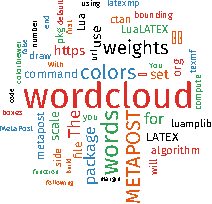
\includegraphics[width=\linewidth]{doc-wc.pdf}
\end{center}

\section{To do}

Some things to do:
\begin{itemize}
  \item Improve intersection of words by using the letters bounding boxes.
  \item Work on speed of the algorithm.
  \item Add supported languages (ignored words).
  \item Improve text file analysis with Lua to build the set of words and
  weights.  
  \item Build wordcloud inside a shape.
  \item Add options for rotation of words.
\end{itemize}

\printbibliography
\printindex
\newpage



\end{document}
